\section{Gaussian process}
Gaussian process is a stochastic process, such that every finite collection of those random variables has a multivariate normal distribution, i.e., every finite linear combination of them is normally distributed.
It is determined by a mean function $m(\bm{x})$ and a covariance function $k(\bm{x},\bm{x}')$,
and we write a sample function as
\begin{align}
    f\sim\mathcal{GP}(m,k).
\end{align}
Functions $m$ and $k$ are characterized by sampled functions as follows:
\begin{align}
    &\mathbb{E}_{f\sim\mathcal{GP}(m,k)}\left[f(\bm{x})\right]=m(\bm{x}),\\
    &\mathbb{E}_{f\sim\mathcal{GP}(m,k)}\left[f(\bm{x})f(\bm{x}')\right]=k(\bm{x},\bm{x}').
\end{align}
The covariance function describes \textit{similarity} of $f$ at point $\bm{x}$ and $\bm{x}'$.
Therefore, the choice of the covariance function is crutial for determining the sampled functions' properties, like stationarity, isotropy, smoothness, and periodicity.
For example, RBF kernel, or squared exponential covariance function, is known to generate a $C^{\infty}$ function with probability one.
Mat\'ern kernel is known to generate a finite-time differentiable function with probability one.
$\min$ function, which is $k(x,x')=\min(x,x')$, corresponds to Browninan motion, and is known to generate non-differentiable functions.
Periodic kernel is known to generate a periodic function.
See Figure~\ref{fig:kernelgp}.

\begin{figure}[htbp]
    \centering
    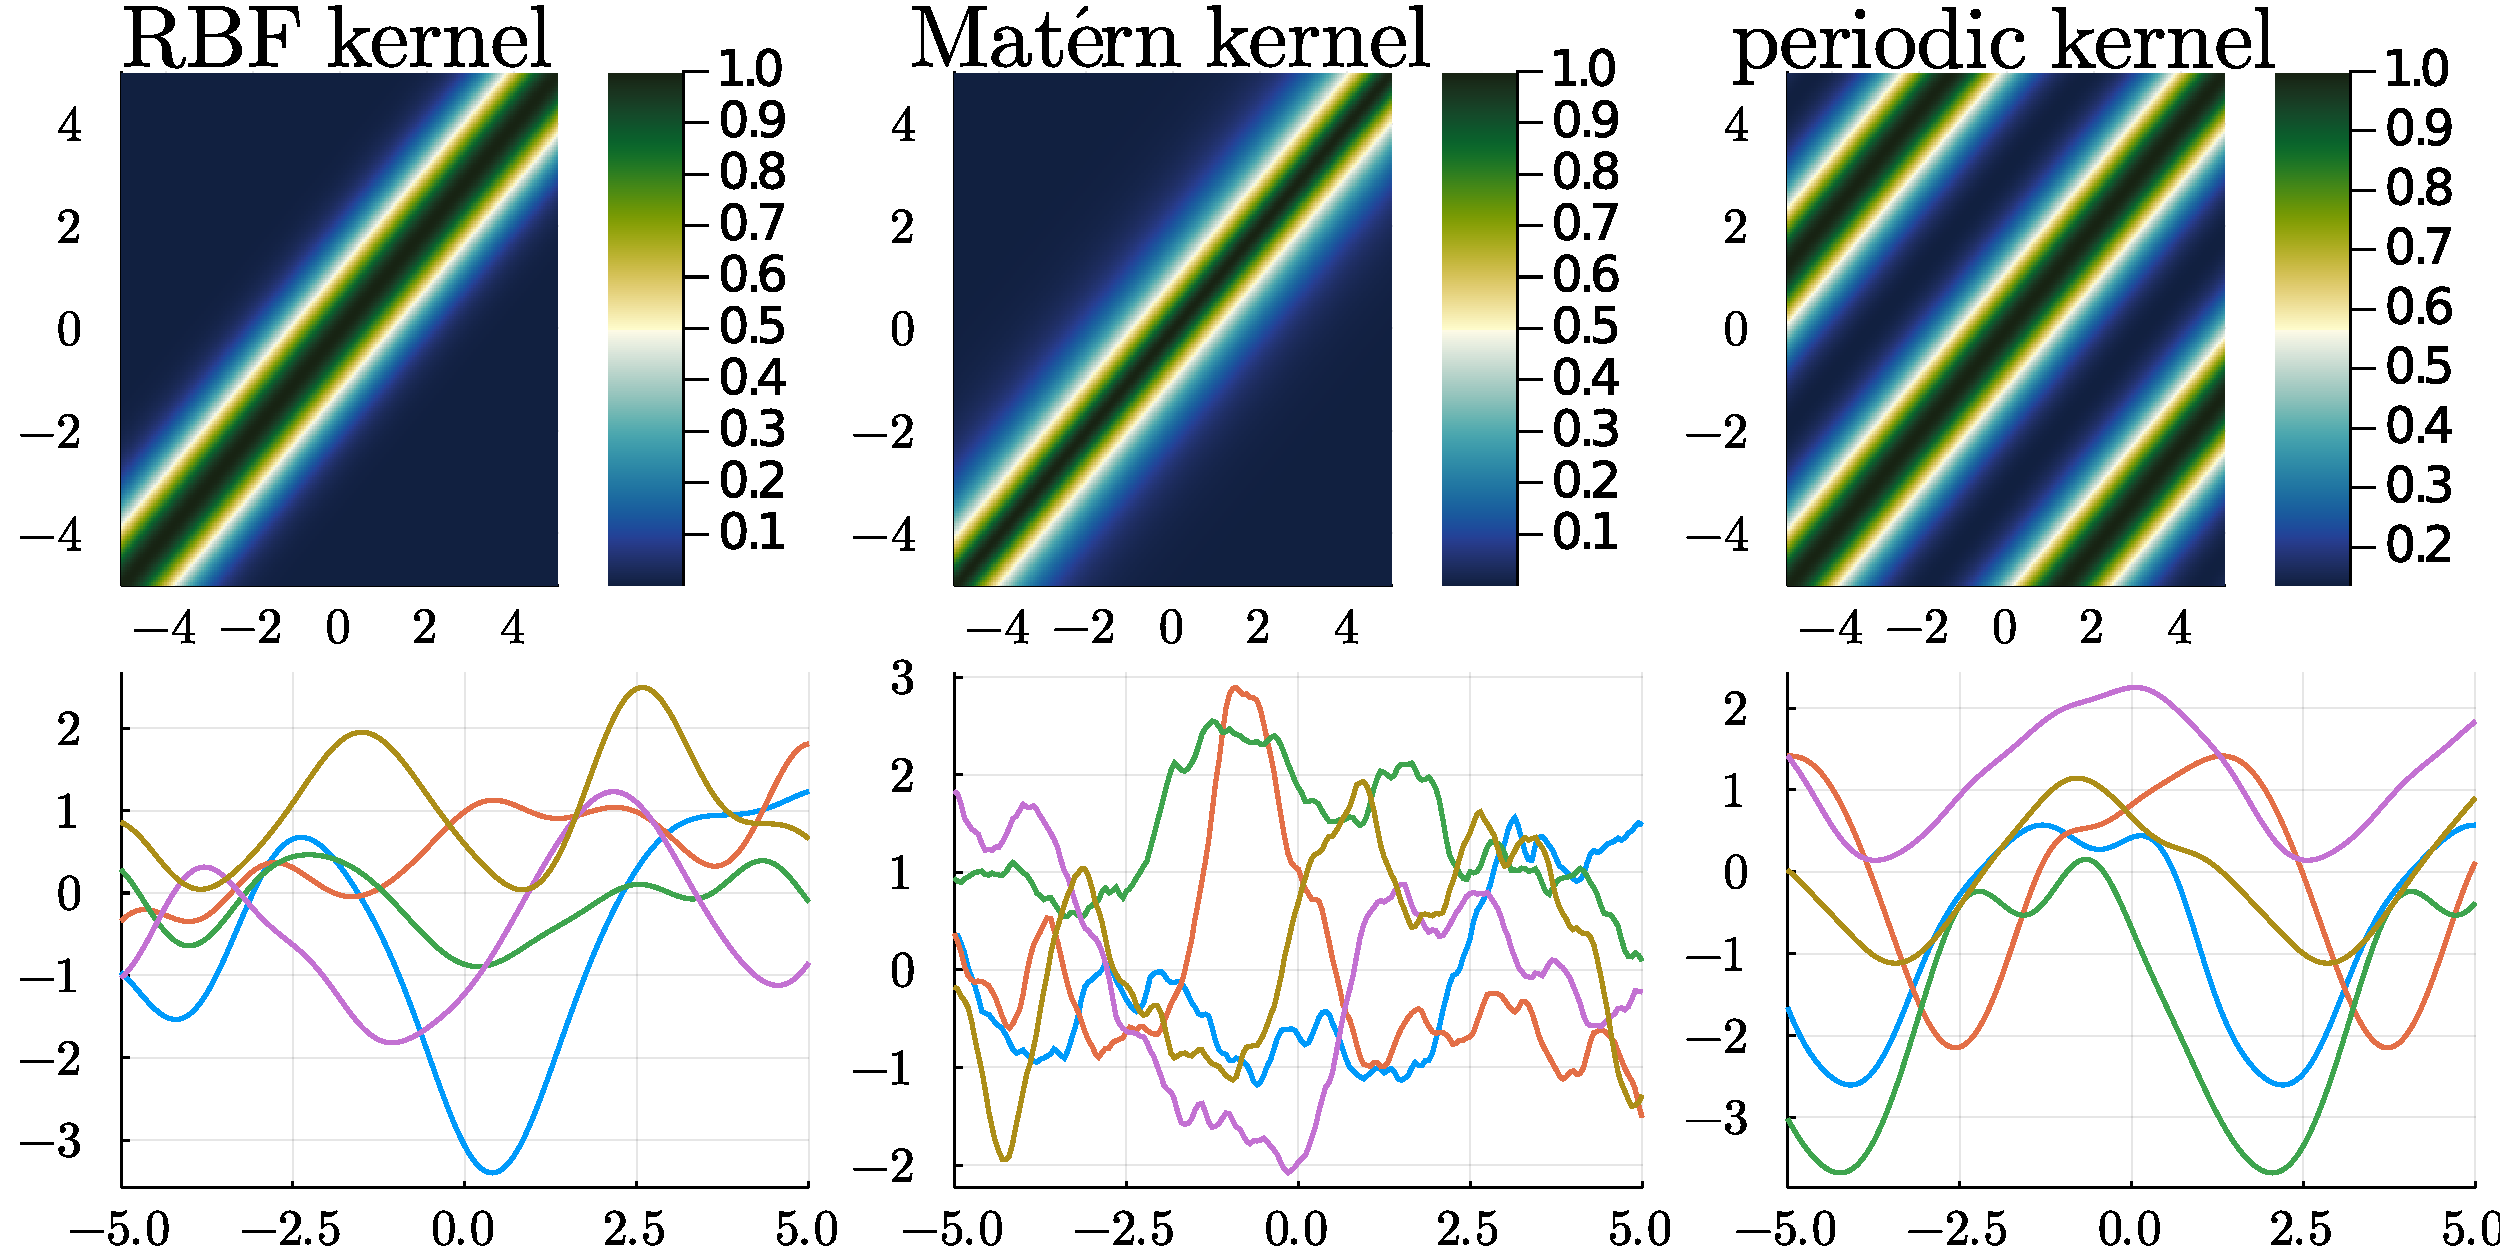
\includegraphics[width=\textwidth]{figs/kernelgp.pdf}
    \caption{Heatmaps of RBF kernel, Mat\'ern kernel, and periodic kernel, and the corresponding Gaussian processes.}
    \label{fig:kernelgp}
\end{figure}

These properties are shown by a complicated functional analysis, and are difficult hence we do not go deep in this note,
but the main idea is to use the \textbf{reproducing kernel Hilbert spaces (RKHS)}.
See the reference hoge for a detailed discussion.

\section{Gaussian process regression}